\documentclass[11pt,a4paper]{ctexart}
\usepackage[margin=2.4cm]{geometry}
\usepackage{amsmath,amssymb,amsthm,mathtools}
\usepackage{xcolor,graphicx,booktabs,array,enumitem,float}
\usepackage[font=small,labelsep=quad]{caption}
\usepackage[colorlinks=true,linkcolor=blue!50!black,citecolor=blue!50!black,urlcolor=blue!50!black]{hyperref}
\setlist{nosep,leftmargin=2em}
\linespread{1.25}

\theoremstyle{definition}
\newtheorem{theorem}{定理}[section]
\newtheorem{proposition}[theorem]{命题}
\newtheorem{lemma}[theorem]{引理}
\newtheorem{corollary}[theorem]{推论}
\theoremstyle{definition}
\newtheorem{numres}[theorem]{数值结果}
\newtheorem{remark}[theorem]{注记}
\renewcommand{\proofname}{证明}

\newcommand{\Usw}{U_{\rm sw}}
\newcommand{\Ssw}{S_{\rm sw}}
\newcommand{\rA}{r_{A'}}
\newcommand{\rhat}{\hat r}
\newcommand{\rloc}{r_{\rm loc}}
\newcommand{\rinf}{r_{\infty}}
\newcommand{\Uglob}{U_{\rm glob}}
\newcommand{\QO}{\mathrm{QO}}
\newcommand{\proven}{\textbf{（已证明）}}
\newcommand{\numer}{\textbf{（数值）}}

\title{阈值策略下成本最优控制的完整结构\\[2pt]\large 全部成本权重下的切换、跳跃与显式解}
\author{成本最优分析专稿（独立于主稿，2026-10-19）}
\date{}

\begin{document}
\maketitle

\begin{abstract}
\noindent 在含接触控制与追踪隔离的无回流 SIQR 模型中，阈值策略把二次干预强度成本 $J$ 的最小化化为逐状态的一维问题。本文对全部权重比 $r=w_q/w_c>0$ 刻画成本最优反馈律 $c_c^*(S)$、$q_c^*(S)$。所有阈值只依赖 $b=(1-\beta)(1-q_0)$。主要结论如下。
\begin{enumerate}
\item 任意权重下，隔离比例在整个阈值控制期内单调不增；若有跳跃，则跳跃时隔离比例与接触率同时下降。$r$ 增大时，控制时长与累计新增感染不减，新增隔离易感者不增，最小成本是 $r$ 的凹增函数。
\item 仅隔离段的起点为 $S_{\rm glob}(r)$。$r\le\rhat(b)=\bigl(\Ssw/(\Ssw-S_c)\bigr)^2$ 时它就是 $\Ssw$，切换连续；$r>\rhat$ 时它严格前移，由显式的相切条件确定，接触率在此处跳变。
\item 成本最优控制在整个控制期连续，当且仅当 $r\le\rA(b)=16/(b+\sqrt{b^2-8b+8})^2$。此时最优控制唯一，并有以隔离水平为参数的显式表达。$\rA(b)\in(2,4)$，所以默认权重 $r=2$ 对一切参数都落在这一情形。
\item $r>\rA$ 时，最优控制至少有一次跳跃（已证明）。数值上恰有一次，所有跳跃点组成一条从尖点出发的单调曲线。每个连续段内控制仍有显式参数表达；作为 $S$ 的函数，它一般没有根式解（伽罗瓦群为 $S_5$）。
\item 推论：$r\le\rA$ 时，能力约束下的成本最优控制就是把无约束的控制截断到允许区间；时长约束下，最小成本 $V(T)$ 是 $T$ 的凸函数，每个允许时长都有匹配的乘子；混合两种措施带来的成本节省、控制时长与感染的增量，都与阈值 $\eta$ 无关。
\end{enumerate}
\noindent 文中标“已证明”的结论给出了完整证明；标“数值”的结论只有数值证据，并写明了所用网格。
\end{abstract}

\tableofcontents

%==========================================================
\section{问题与记号}
\label{sec:setup}

\subsection{逐状态问题}
沿用主稿第 4、5 章的设定（无回流模型，不考虑能力约束，第~\ref{sec:capacity}~节除外）。阈值控制期内 $I\equiv\eta$。控制由接触率的状态函数 $c_c(S)$ 决定，满足 $c_0S_c/S\le c_c(S)\le c_0$；隔离比例为 $q_c(S)=1-c_0(1-q_0)S_c/(c_c(S)S)$。易感者满足 $\dot S=-(\eta/N)[c_c(S)S-c_0\bar S]$，其中
\[
S_c=\frac{\gamma N}{\beta c_0(1-q_0)},\qquad \bar S=\frac{(1-\beta)\gamma N}{\beta c_0}<S_c .
\]
二次干预强度成本 $J=\int_{t_1}^{t_2}\bigl[w_c((c_0-c)/c_0)^2+w_q((q-q_0)/(1-q_0))^2\bigr]dt$ 可以写成对 $S$ 的积分：
\[
J[c_c]=\frac{N}{\eta}\int_{S_c}^{S^*}f(S,c_c(S))\,dS ,\qquad f(S,c)=\frac{w_c(1-c/c_0)^2+w_q\bigl(1-\frac{c_0S_c}{cS}\bigr)^2}{cS-c_0\bar S}.
\]

\subsection{无量纲化}
记
\[
U=\frac{S}{S_c},\qquad u=\frac{cS}{c_0S_c}=\frac{1-q_0}{1-q},\qquad b=\frac{\bar S}{S_c}=(1-\beta)(1-q_0)\in(0,1),\qquad r=\frac{w_q}{w_c},\qquad \theta=\frac{\eta}{N}.
\]
$u$ 是隔离水平的单调变换：$u=1$ 即 $q=q_0$（仅减少接触），$u=U$ 即 $c=c_0$（仅隔离控制）。于是
\[
\frac{c}{c_0}=\frac uU,\qquad \frac{q-q_0}{1-q_0}=1-\frac1u,\qquad \dot U=-c_0\theta\,(u-b),
\]
\begin{gather}
\Delta t=\frac{1}{c_0\theta}\int_1^{U^*}\frac{dU}{u(U)-b},\qquad
J=\frac{w_c}{c_0\theta}\int_1^{U^*}G\bigl(u(U);U\bigr)\,dU,\notag\\
G(u;U)=\frac{(1-u/U)^2+r(1-1/u)^2}{u-b},
\label{eq:G}
\end{gather}
允许集合为 $1\le u(U)\le U$。由主稿定理 5.1，最小化 $J$ 等价于对每个 $U$ 最小化 $G(\cdot;U)$。

\begin{lemma}[与阈值无关]\label{lem:invariance}\proven
逐状态最小点 $u^*(U)$ 只依赖 $(b,r)$ 与 $U$。$\eta$、$S_0$、$I_0$ 只通过积分上限 $U^*=S^*/S_c$ 和系数 $1/(c_0\theta)$ 进入 $\Delta t$ 与 $J$。
\end{lemma}

\subsection{分解与切换状态的机制}
记 $C_U(u)=(1-u/U)^2/(u-b)$，$h(u)=r(1-1/u)^2/(u-b)$，则 $G=C_U+h$。接触项 $C_U$ 在 $u=U$ 处有二重零点；隔离项 $h$ 与状态无关，且
\begin{equation}
h'(u)=-\frac{r(u-1)(u^2-3u+2b)}{u^3(u-b)^2}.
\label{eq:hprime}
\end{equation}
所以 $h$ 在 $[1,\Usw]$ 上增、在 $[\Usw,\infty)$ 上严格减，其中
\[
\Usw=\frac{\Ssw}{S_c}=\frac{3+\sqrt{9-8b}}{2}\in(2,3).
\]
$h(U)$ 是仅隔离控制在状态 $U$ 上每移出一名易感者所付的成本（差一个常数因子），$\Ssw$ 正是它的峰值点。因为 $h\propto r$，峰值位置与权重无关。下面还反复用到交叉导数
\begin{equation}
\frac{\partial^2G}{\partial u\,\partial U}=-\frac{2\,(u^2-2bu+bU)}{U^3(u-b)^2}<0 ,
\label{eq:cross}
\end{equation}
其中 $u^2-2bu+bU=(u-b)^2+b(U-b)>0$。

\subsection{参数化与阈值一览}
令 $t=\Usw\in(2,3)$，则 $b=t(3-t)/2$。全文出现的权重阈值都只依赖 $b$（或 $t$），见表~\ref{tab:thr-formula}。

\begin{table}[htbp]\centering\small
\caption{权重阈值与特征状态（$t=\Usw$，$b=t(3-t)/2$）}\label{tab:thr-formula}
\begin{tabular}{@{}llll@{}}\toprule
记号 & 含义 & 公式 & 取值范围\\\midrule
$\Usw$ & 仅隔离控制局部最优的分界 & $(3+\sqrt{9-8b})/2$ & $(2,3)$\\
$U_c$ & 尖点状态（连续性失去处） & $b+\sqrt{b^2-8b+8}$ & $(2,2\sqrt2)$\\
$\rA$ & 整段连续的最大权重比 & $16/U_c^2$ & $(2,4)$\\
$\rhat$ & 切换开始离开 $\Ssw$ & $t^2/(t-1)^2$ & $(9/4,4)$\\
$\rloc$ & $\Ssw$ 处的二阶（局部）阈值 & $t^2/(2t-3)$ & $(3,4)$\\
$\rinf$ & 内部驻点曲线断开 & $27/(9-8b)=27/(2t-3)^2$ & $(3,27)$\\
$r_C(U^*)$ & 仅隔离段在一次疫情中消失 & 式~\eqref{eq:tangent} 中取 $U=U^*$ & 依赖 $U^*$\\\bottomrule
\end{tabular}
\end{table}

\begin{proposition}[阈值的次序]\label{prop:order}\proven
对一切 $b\in(0,1)$ 有 $U_c<\Usw$ 和 $2<\rA<\rhat<\rloc<\rinf$。$\rA$ 与 $\rhat$ 关于 $b$ 严格递增；$b\to0$ 时 $\rA\to2$、$\rhat\to9/4$，$b\to1$ 时二者都趋于 $4$。
\end{proposition}
\begin{proof}
各项比较都化为 $t\in(2,3)$ 上的多项式符号：
\begin{itemize}
\item $U_c<t$ 等价于 $8-8b<t^2-2tb$，即 $(t-2)^3>0$；
\item $\rA<\rhat$ 等价于 $U_c>4(t-1)/t$，平方后化为 $(t-1)(t-2)^2>0$（右端非正时显然成立）；
\item $\rhat<\rloc$ 等价于 $2t-3<(t-1)^2$，即 $(t-2)^2>0$；
\item $\rloc<\rinf$ 等价于 $t^2(2t-3)<27$，而左端在 $(2,3)$ 上递增且 $t=3$ 时等于 $27$。
\end{itemize}
$\rA>2$ 等价于 $U_c<2\sqrt2$，由 $dU_c/db=1+(b-4)/\sqrt{b^2-8b+8}<0$ 及 $U_c(0)=2\sqrt2$ 得到；单调性与极限直接计算可得。
\end{proof}

%==========================================================
\section{逐状态问题的结构}
\label{sec:pointwise}

\begin{proposition}[端点]\label{prop:endpoints}\proven
对每个 $U>1$：
\begin{itemize}
\item $G_u(1;U)<0$，所以 $u=1$（仅减少接触）从不是局部最小点；
\item $G_u(U;U)=h'(U)$，所以 $u=U$（仅隔离控制）在 $U>\Usw$ 时是严格局部最小点，在 $U<\Usw$ 时不是局部最小点。
\end{itemize}
\end{proposition}
\begin{proof}
$G_u(1;U)=-\dfrac{2(1-1/U)}{U(1-b)}-\dfrac{(1-1/U)^2}{(1-b)^2}<0$。$C_U$ 在 $u=U$ 处有二重零点，故 $G_u(U;U)=h'(U)$，再由式~\eqref{eq:hprime} 得结论。这就是主稿命题 5.3。
\end{proof}

\begin{proposition}[内部驻点的显式参数化]\label{prop:branch}\proven
令 $v=1-u/U$（接触降幅）。$G_u(u;U)=0$ 等价于
\begin{equation}
F(u,v):=(u-2b)v^2-2(u-b)v+C(u)=0,\qquad C(u)=r\,\frac{(u-1)(3u-u^2-2b)}{u^2}.
\label{eq:F}
\end{equation}
内部驻点只可能出现在 $u\in(1,\Usw)$ 且 $C(u)<u$ 处；在这样的 $u$ 上，$(0,1)$ 内恰有一个根
\begin{equation}
v_s(u)=\frac{C(u)}{(u-b)+\sqrt{(u-b)^2-(u-2b)C(u)}},
\label{eq:vs}
\end{equation}
它对应的状态为
\[
U_s(u)=\frac{u}{1-v_s(u)} .
\]
因此全部内部驻点组成一条显式曲线 $\{(u,U_s(u))\}$，在该曲线上
\[
q=1-\frac{1-q_0}{u},\qquad c=c_0\bigl(1-v_s(u)\bigr),\qquad S=S_cU_s(u).
\]
条件 $C(u)<u$ 对一切 $u\in(1,\Usw)$ 成立，当且仅当 $r<\rinf(b)=27/(9-8b)$。$r\ge\rinf$ 时曲线在 $u=3/2$ 附近断开，断点两侧 $U_s\to\infty$。
\end{proposition}
\begin{proof}
把 $U=u/(1-v)$ 代入 $G_u$ 的分子并乘以 $u$，即得式~\eqref{eq:F}。下面看 $(0,1)$ 内的根。
\begin{itemize}
\item $u\ge\Usw$ 时 $C(u)\le0$。由于 $u>2>2b$，两根之积 $C/(u-2b)\le0$，而 $F(u,1)=C-u<0$，所以正根大于 $1$，$(0,1)$ 内无根。
\item $1<u<\Usw$ 时 $C>0$，故 $F(u,0)=C>0$。若 $u>2b$，抛物线开口向上，顶点 $(u-b)/(u-2b)>1$，所以 $(0,1)$ 内有根当且仅当 $F(u,1)=C-u<0$，且此时恰有一个根（较小根）。$u\le2b$ 时同理。
\end{itemize}
把较小根有理化即得式~\eqref{eq:vs}。最后，$C(u)<u$ 等价于 $r\varphi(u)<1$，其中 $\varphi(u)=(u-1)(3u-u^2-2b)/u^3$；由 $\varphi'(u)=-2(2u-3)(u-b)/u^4$，$\varphi$ 的最大值为 $\varphi(3/2)=(9-8b)/27$。
\end{proof}

\begin{proposition}[局部最小与曲线方向]\label{prop:minmax}\proven
在内部驻点 $(u,U_s(u))$ 上，$G_{uu}=-G_{uU}\,U_s'(u)$。由式~\eqref{eq:cross}，该驻点是严格局部最小点当且仅当 $U_s'(u)>0$，是局部最大点当且仅当 $U_s'(u)<0$。
\end{proposition}
\begin{proof}
对恒等式 $G_u(u,U_s(u))\equiv0$ 求导即得。
\end{proof}

\begin{proposition}[折叠判据]\label{prop:fold}\proven
记 $\tilde F=u^2F$，$\tilde H=(1-v)\tilde F_v-u\tilde F_u$，则沿驻点曲线 $\operatorname{sign}U_s'(u)=-\operatorname{sign}\tilde H(u,v_s(u))$，并且
\begin{gather}
\operatorname{Res}_v(\tilde F,\tilde H)=4u^4(u-b)^2P(u,b,r),\notag\\
P=\bigl(rX+u^3\bigr)^2-4rb^2u^2(2u-3),\qquad X=u^3-6u^2+6u+2b(3u-4).
\label{eq:P}
\end{gather}
两个多项式的首项系数 $u^2(u-2b)$ 与 $-u^2(5u-8b)$ 在 $u>0$ 时不同时为零，所以 $P\neq0$ 蕴含 $\tilde H(u,v_s)\neq0$。
\end{proposition}
\begin{proof}
$dU_s/du=[(1-v)F_v-uF_u]/(F_v(1-v)^2)$，且沿较小根有 $F_v=-2\sqrt{(u-b)^2-(u-2b)C}<0$。结式由符号计算得到。
\end{proof}

\begin{remark}[作为 $S$ 的函数没有根式解]\label{rem:galois}
内部最优点是 $u$ 的五次方程（主稿式 5.4）的根。在 $(b,r,U)=(\tfrac12,2,2)$、$(\tfrac45,2,\tfrac95)$、$(\tfrac35,2,\tfrac{11}5)$、$(\tfrac45,\tfrac{16}5,\tfrac94)$、$(\tfrac12,5,3)$ 五个有理点上，该五次式不可约，伽罗瓦群都是 $S_5$。所以 $c_c^*$ 一般不能写成 $S$ 的根式表达。命题~\ref{prop:branch} 给出的是另一种“解析解”：以隔离水平 $u$ 为参数，$(c,q,S)$ 都显式。
\end{remark}

%==========================================================
\section{对任意权重成立的单调性}
\label{sec:monotone}

\begin{theorem}[单调比较静态]\label{thm:monotone}\proven
设 $r>0$ 任意，$u^*$ 是逐状态最小点的任一选择。
\begin{enumerate}[label=(\roman*)]
\item 若 $U_1<U_2$，则 $u^*(U_1)\le u^*(U_2)$。因此 $q_c^*(S)$ 随 $S$ 不减，即在整个阈值控制期内随时间不增。在任一跳跃处，沿时间方向 $u$ 向下跳，隔离比例与接触率 $c/c_0=u/U$ 同时下降，控制由偏重隔离转为偏重减少接触。
\item 若 $r_1<r_2$，则在每个状态上 $u^*(U;r_2)\le u^*(U;r_1)$，即 $c^*$、$q^*$ 都不增。因此：
\begin{itemize}
\item 控制时长 $\Delta t(r)$ 与控制期累计新增感染 $\beta(S^*-S_c)+(1-\beta)\gamma\eta\Delta t$ 随 $r$ 不减；
\item 新增隔离易感者人数 $(1-\beta)(S^*-S_c-\gamma\eta\Delta t)$ 随 $r$ 不增；
\item 最小成本 $J_{\min}(r)$ 是 $r$ 的凹增函数，最优解中的隔离二次分项 $\int(1-1/u^*)^2dt$ 随 $r$ 不增。
\end{itemize}
\end{enumerate}
\end{theorem}
\begin{proof}
(i) 设 $u_2:=u^*(U_2)<u_1:=u^*(U_1)$。此时 $u_2<u_1\le U_1$，两点在两个状态上都允许。由最优性，
\[
[G(u_1;U_2)-G(u_2;U_2)]-[G(u_1;U_1)-G(u_2;U_1)]\ge0 ,
\]
但左端等于 $\int_{U_1}^{U_2}\!\int_{u_2}^{u_1}G_{uU}\,du\,dU<0$（式~\eqref{eq:cross}），矛盾。

(ii) 写 $G=A(u;U)+rB(u)$，$B=(1-1/u)^2/(u-b)$。两个最优性不等式相加得 $(r_2-r_1)[B(u_2)-B(u_1)]\le0$，即 $B(u_2)\le B(u_1)$。由命题~\ref{prop:endpoints}、\ref{prop:branch}，最优点只能在 $(1,\Usw)$ 或等于 $U$；而 $B$ 在 $[1,\Usw]$ 上严格增。
\begin{itemize}
\item 若 $u_1,u_2\in(1,\Usw)$，则 $u_2\le u_1$；
\item 若 $u_1=U$，结论显然；
\item 若 $u_2=U$，由定理~\ref{thm:upper}(b)，仅隔离控制在 $r_1$ 下是唯一最优点，故 $u_1=U$。
\end{itemize}
时长与感染的结论由 $\Delta t$ 关于 $u$ 递减、以及主稿定理 4.5 中的仿射关系得到。$J_{\min}/w_c=\min_c\{\int A+r\int B\}$ 是一族仿射函数的下确界，所以是凹函数；$\int B\ge0$ 使它不减；最优解的 $\int B$ 是凹函数的超梯度，随 $r$ 不增。
\end{proof}

%==========================================================
\section{仅隔离段：切换状态与第一个权重阈值}
\label{sec:front}

\begin{theorem}[上集性]\label{thm:upper}\proven
记 $\Omega=\{(U,r):\ u=U\ \text{是}\ G(\cdot;U)\ \text{的全局最小点}\}$。
\begin{enumerate}[label=(\alph*)]
\item 若 $(U_0,r)\in\Omega$，则对一切 $U_1>U_0$，$u=U_1$ 是唯一全局最小点。
\item 若 $(U,r_2)\in\Omega$ 且 $r_1<r_2$，则 $u=U$ 在 $r_1$ 下是唯一全局最小点。
\end{enumerate}
因此存在 $\Uglob(r)\ge\Usw$：仅隔离控制在 $U>\Uglob(r)$ 上是唯一最优点，在 $1<U<\Uglob(r)$ 上不是最优点。$\Uglob(r)$ 有限、连续，并随 $r$ 不减。
\end{theorem}
\begin{proof}
(a) 由命题~\ref{prop:endpoints} 有 $U_0\ge\Usw$。分两种情形：
\begin{itemize}
\item $u\le U_0$：$C_{U_1}(u)+h(u)>C_{U_0}(u)+h(u)\ge h(U_0)\ge h(U_1)$，因为 $C_U(u)$ 关于 $U$ 严格增，而 $h$ 在 $[\Usw,\infty)$ 上递减；
\item $U_0<u<U_1$：$C_{U_1}(u)+h(u)\ge h(u)>h(U_1)$。
\end{itemize}
(b) $G(u;U)-G(U;U)=C_U(u)+r[h_1(u)-h_1(U)]$，$h_1=h/r$。对 $h_1(u)<h_1(U)$ 的 $u$，减小 $r$ 使差值严格变大；对 $h_1(u)\ge h_1(U)$ 的 $u$，差值不小于 $C_U(u)>0$。

有限性：$u<\Usw$ 时 $C_U(u)\ge(1-\Usw/U)^2/(\Usw-b)$ 有正下界；$u\in[\Usw,U)$ 时 $h(u)>h(U)$；而 $h(U)<r/(U-b)\to0$。

连续性：$\Omega$ 是闭集，所以 $\Uglob$ 下半连续；又因 $\Uglob$ 单调，它左连续。若 $\Uglob(r+)>\Uglob(r)=U_0$，取 $U\in(U_0,\Uglob(r+))$。由 (a)，$U$ 是严格的唯一最小点；又 $G_u(U;U)=h'(U)<0$，这一严格性在 $r$ 的小扰动下保持，与 $(U,r')\notin\Omega$ 矛盾。
\end{proof}

\begin{theorem}[第一个权重阈值]\label{thm:rhat}\proven
$\Uglob(r)=\Usw$ 当且仅当
\[
r\le\rhat(b)=\Bigl(\frac{\Usw}{\Usw-1}\Bigr)^2=\Bigl(\frac{3+\sqrt{9-8b}}{1+\sqrt{9-8b}}\Bigr)^2\in\bigl(\tfrac94,4\bigr).
\]
$r<\rhat$ 时，成本最优控制在 $\Ssw$ 处连续地离开仅隔离控制。$r=\rhat$ 时，在 $\Ssw$ 上仅隔离控制与内部点 $c/c_0=\hat x:=1/(\Usw-1)$ 等值。
\end{theorem}
\begin{proof}
令 $x=u/U=c/c_0$，$\sigma=1/U$，$A=(1-\sigma)^2$，$B=1-b\sigma$。对 $x\in[\sigma,1)$，$G(xU;U)\ge G(U;U)$ 等价于
\[
Q(x):=B(1-x)x^2+rR(x)\ge0,\qquad R(x)=Ax^2-B\sigma(2-\sigma)x+B\sigma^2 ,
\]
这里用到恒等式 $B(x-\sigma)^2-Ax^2(x-b\sigma)=(1-x)R(x)$。

在 $\sigma_{\rm sw}=1/\Usw$ 上有 $2b\sigma^2-3\sigma+1=0$，即 $2\sigma B=1-\sigma$，于是 $R=A(x-1)(x-x_2)$，$x_2=\sigma/[2(1-\sigma)]<\sigma$。这样 $Q=(1-x)[Bx^2-rA(x-x_2)]$，条件化为 $r\le(B/A)x^2/(x-x_2)$。右端在 $x=2x_2\in(\sigma,1)$ 处取最小值 $4x_2B/A=1/(1-\sigma)^2$。

$r<\rhat$ 时，$Q>0$ 在 $[\sigma,1)$ 上成立，故 $(\Usw,r)\in\Omega$ 且最小点唯一；又 $U<\Usw$ 时仅隔离控制不是局部最小点，所以 $\Uglob=\Usw$。由 Berge 极大值定理，最小点在 $\Usw$ 处连续。$r>\rhat$ 时 $(\Usw,r)\notin\Omega$，由定理~\ref{thm:upper} 得 $\Uglob>\Usw$。
\end{proof}

\begin{theorem}[$r>\rhat$ 时的切换状态]\label{thm:tangent}\proven
$r>\rhat$ 时，$U=\Uglob(r)>\Usw$ 由相切等值条件确定：存在 $\hat u\in\bigl(\tfrac{2U}{2U-1},U\bigr)$，使
\begin{equation}
r=\frac{\hat u^3}{(2U-1)\hat u-2U},\qquad (U-1)^2\hat u^3=2(U-b)\bigl[(2U-1)\hat u^2-U(U+1)\hat u+U^2\bigr].
\label{eq:tangent}
\end{equation}
等价地，$(U,\hat u)\mapsto(r,b)$ 给出切换曲线的有理参数化：$b=U-(U-1)^2\hat u^3/\bigl(2[(2U-1)\hat u^2-U(U+1)\hat u+U^2]\bigr)$。

对给定的 $(U,b)$，第二式是 $\hat u$ 的三次方程。记 $r_g(U,b)$ 为由其合格根给出的 $r$ 的最小值，则 $\Uglob(r)$ 是 $r_g(U,b)=r$ 的解。在 $S_{\rm glob}$ 处，接触率由 $c_0$ 跳到 $c_0\hat u/U$；$r\downarrow\rhat$ 时，跳变幅度趋于 $1-\hat x=1-1/(\Usw-1)>0$。$\Uglob(r)$ 关于 $r>\rhat$ 严格增，并且
\[
\Uglob(r)\ \ge\ b+r(1-b),\qquad\text{即}\qquad S_{\rm glob}\ \ge\ \bar S+r(S_c-\bar S).
\]
\end{theorem}
\begin{proof}
相切等值即 $G_u(\hat u;U)=0$ 且 $G(\hat u;U)=G(U;U)$。对 $(r,b)$ 解这两个方程得式~\eqref{eq:tangent}，并由符号计算回代核对。下界来自与 $u=1$ 的比较：$G(U;U)\le G(1;U)$ 等价于 $r/(U-b)\le1/(1-b)$。

严格单调：若 $\Uglob(r_1)=\Uglob(r_2)=U_0>\Usw$ 且 $r_1<r_2$，由定理~\ref{thm:upper}(b)，$U_0$ 在 $r_1$ 下是严格唯一最小点，按连续性论证，稍小于 $U_0$ 的状态也属于 $\Omega$，矛盾。跳变幅度的极限：$r\downarrow\rhat$ 时，$\hat u/U\to2x_2=1/(\Usw-1)$。
\end{proof}

\begin{corollary}[一次疫情中仅隔离段的消失]\label{cor:C}\proven
设 $U^*=S^*/S_c>\Usw$。阈值控制期内存在仅隔离段，当且仅当 $r<r_C:=r_g(U^*,b)$。$r\ge(U^*-b)/(1-b)$ 是仅隔离段消失的显式充分条件。仅隔离段的时长为 $\frac{1}{c_0\theta}\ln\frac{U^*-b}{\Uglob(r)-b}$。
\end{corollary}

\begin{remark}[局部阈值不决定全局切换]
$\Ssw$ 处的二阶条件给出 $\rloc=t^2/(2t-3)$：$r<\rloc$ 时，内部驻点曲线在 $u=\Usw$ 处递增（$U_s'(\Usw)=1-r/\rloc$）。由命题~\ref{prop:order}，$\rloc>\rhat$，所以切换在局部失稳之前就已离开 $\Ssw$，原因是另一个内部极小点的值先追上了端点值。基准参数下 $\rloc=3.353$、西安参数下 $3.097$，与早先由 $g_{xx}(1)=0$ 算得的 3.35、3.10 一致。
\end{remark}

%==========================================================
\section{内部段：连续性的充要条件与尖点}
\label{sec:interior}

\begin{theorem}[连续性]\label{thm:continuity}\proven
记 $U_c(b)=b+\sqrt{b^2-8b+8}$，$\rA(b)=16/U_c^2$。
\begin{enumerate}[label=(\roman*)]
\item 若 $0<r\le\rA(b)$，则对每个 $U>1$，$G(\cdot;U)$ 在 $[1,U]$ 上单峰：$U<\Usw$ 时先严格减、后严格增，$U\ge\Usw$ 时严格减。因此：
\begin{itemize}
\item 成本最优控制唯一，且在 $[S_c,\infty)$ 上连续；
\item $S\ge\Ssw$ 时它等于仅隔离控制；
\item $S_c<S<\Ssw$ 时它由命题~\ref{prop:branch} 的参数式给出，$u\in(1,\Usw)$，且 $U_s$ 严格增。
\end{itemize}
\item 若 $r>\rA(b)$，则 $U_s'(2)<0$，即内部驻点曲线在隔离水平 $u=2$（$q=(1+q_0)/2$）处折叠。成本最优反馈律在 $(S_c,\infty)$ 上至少有一次跳跃：$r<\rhat$ 时跳跃位于 $(S_c,\Ssw)$；$r\ge\rhat$ 时跳跃位于 $S_{\rm glob}(r)$。
\item 尖点位于 $(U,r)=(U_c,\rA)$。尖点处 $c/c_0=2/U_c=\sqrt{\rA}/2$，$q=(1+q_0)/2$。
\end{enumerate}
默认权重 $r=2$ 对一切参数都满足 (i)；由 $\rA(0+)=2$，常数 $2$ 不能对一切 $b$ 一致地改进。
\end{theorem}

\begin{proof}
\textbf{第一步：$r<\rA$ 时 $P>0$。}

\emph{情形 $u\le3/2$。} 记 $W=rX+u^3$，则 $P=W^2+4rb^2u^2(3-2u)$。$u<3/2$ 时第二项为正。$u=3/2$ 时 $W=27/8-r(9/8-b)>0$，因为 $r<\rA<\rinf=27/(9-8b)$。

\emph{情形 $u>3/2$。} 令 $w=\sqrt{2u-3}$，$s=\sqrt r$，则 $P=F_1F_2$，其中
\[
F_1=s^2X+u^3-2sbuw,\qquad F_2=F_1+4sbuw .
\]
令 $s_A=\sqrt{\rA}$，它满足 $(1-b)s_A^2+bs_A-2=0$，即 $b=(s_A^2-2)/(s_A(s_A-1))$。代入后符号计算给出
\[
F_1\big|_{s=s_A}=\frac{(w-1)^2\,Q(w,s_A)}{8(s_A-1)},
\]
\[
Q=(s-1)(s^2+1)w^3(w+2)+12(s-1)w^2-2(s^3+3s^2-11s+3)w+(-s^3+9s^2+11s-27).
\]
在 $s\in(\sqrt2,2)$ 上，常数项 $\ge3.728$（在 $\sqrt2$ 处取最小值，且递增），一次项系数 $\ge-2$（在 $s=2$ 处取最小值，且递减），二次项系数 $\ge12(\sqrt2-1)>4.97$，三、四次项非负。所以对 $w\ge0$，
\[
Q\ge3.728-2w+4.97w^2>0 .
\]
故 $F_1(\cdot;s_A)\ge0$，等号只在 $w=1$（$u=2$）处成立。

对 $s<s_A$ 的推广：$F_1$ 是 $s$ 的二次式。
\begin{itemize}
\item 若 $X\le0$，$F_1$ 在 $s>0$ 上严格减，故 $F_1(s)>F_1(s_A)\ge0$。
\item 若 $X>0$ 且 $F_1$ 有实根 $s_1\le s_2$，则 $X\le b^2w^2/u$，于是
\[
s_2\ge\frac{buw}{X}\ge\frac{u^2}{bw}>\frac{u^2}{\sqrt{2u-3}}\ge4>s_A .
\]
又 $F_1(s_A)\ge0$，所以 $s_A\le s_1$，从而 $s<s_A$ 时 $F_1>0$。
\item 若 $F_1$ 没有实根，则 $F_1>0$。
\end{itemize}
最后，$F_2>F_1>0$，故 $P>0$。

\textbf{第二步：$r\le\rA$ 时曲线单调。} $r<\rA$ 时 $P>0$，由命题~\ref{prop:fold}，$\tilde H(u,v_s)\neq0$。$r\to0$ 时 $\tilde H\to-2u^2(u-b)<0$，且它关于 $r$ 连续（$r<\rinf$，曲线不断开），故 $\tilde H<0$，即 $U_s'>0$。$r=\rA$ 时，取极限得 $\tilde H\le0$，零点只在 $u=2$，所以 $U_s$ 仍严格增。

\textbf{第三步：单峰性。} $U_s$ 是 $(1,\Usw)\to(1,\Usw)$ 的严格增双射。对 $U<\Usw$，恰有一个内部驻点；再由命题~\ref{prop:endpoints}，$G_u(1)<0<G_u(U)$，所以 $G$ 先减后增。对 $U\ge\Usw$，没有内部驻点，且 $G_u(1)<0$，所以 $G$ 严格减。唯一性与连续性由此得到；参数式即命题~\ref{prop:branch}。

\textbf{第四步：$r>\rA$ 时 $u=2$ 处折叠。} 在 $u=2$ 上，$C(2)=r(1-b)/2$，曲线存在当且仅当 $r<4/(1-b)$；而 $\rhat<4\le4/(1-b)$。$\tilde H$ 对 $F$ 取余后化为 $v$ 的一次式，得
\[
\tilde H(2,v_s)=\frac{4(2-b)}{1-b}\,T,\qquad T=(1-b)(r-2)-2bv_s(2).
\]
$T=0$ 时，$v=(1-b)(r-2)/(2b)$ 必须满足 $F(2,v)=0$，消元后得
\[
\bigl[(1-b)s^2+bs-2\bigr]\bigl[(1-b)s^2-bs-2\bigr]=0 .
\]
第二个因子的根给出 $v=(s+2)/2>1$，不是 $v_s$。所以 $T$ 在 $(0,4/(1-b))$ 上只在 $r=\rA$ 处为零。又 $T(0+)<0$，且 $r\to4/(1-b)$ 时 $T\to2>0$，故 $r>\rA$ 时 $T>0$，即 $U_s'(2)<0$。

\textbf{第五步：$r>\rA$ 时必有跳跃。} 若 $r\ge\rhat$，由定理~\ref{thm:tangent}，$S_{\rm glob}$ 处有跳跃（左极限是内部点 $\hat u<U$）。若 $\rA<r<\rhat$，设最优选择 $u^*$ 在 $(1,\Usw)$ 上连续：
\begin{itemize}
\item 它在每点都是内部驻点，所以 $U_s(u^*(U))=U$，$u^*$ 连续且单射，因而严格增；
\item $u^*\to1$（$U\to1$），且由定理~\ref{thm:rhat}，$u^*\to\Usw$（$U\to\Usw$）。
\end{itemize}
于是 $u^*$ 是 $(1,\Usw)$ 到自身的增双射，$U_s=(u^*)^{-1}$ 严格增，与 $U_s'(2)<0$ 矛盾。

\textbf{第六步：尖点。} 在 $u=2$、$r=\rA$ 处直接验证 $P=P_u=0$。由 $F(2,v)=0$ 解得 $v_c=(2-s_A)/2$，故 $U_c=2/(1-v_c)=4/s_A$。
\end{proof}

\begin{corollary}[显式解]\label{cor:explicit}\proven
$r\le\rA(b)$ 时，成本最优控制为
\begin{align*}
S\ge\Ssw:&\quad c=c_0,\qquad q=1-\frac{\gamma N}{\beta c_0S};\\
S_c<S<\Ssw:&\quad \Bigl(q,\ \frac{c}{c_0},\ \frac S{S_c}\Bigr)=\Bigl(1-\frac{1-q_0}{u},\ 1-v_s(u),\ \frac{u}{1-v_s(u)}\Bigr),\qquad u\in(1,\Usw).
\end{align*}
时间轨迹由 $t-t_1=\frac{1}{c_0\theta}\int_U^{U^*}\frac{dU'}{u^*(U')-b}$ 给出，其中仅隔离段的时长为 $\frac{1}{c_0\theta}\ln\frac{U^*-b}{\Usw-b}$。

两个直接推论：
\begin{itemize}
\item 退出附近 $v_s\approx r(u-1)$，$U_s\approx1+(1+r)(u-1)$，所以 $(1-c/c_0)/(1-S_c/S)\to r/(1+r)$，这就是主稿命题 5.4；
\item $b=0$ 时完全显式：$S/S_c=u^2/\sqrt{(1+r)u^2-4ru+3r}$。
\end{itemize}
\end{corollary}

\begin{numres}[$r>\rA$ 时恰有一次跳跃]\label{num:onejump}\numer
在 14 个 $b$ 值（$0.02$–$0.98$，含两组算例）和每个 $b$ 下约 118 个 $r$ 值（$0.05$–$300$，在 $[\rA,\rhat]$ 附近加密）上，对 $U\in(1,\max\{1.25\Uglob,4\}]$ 的 6000 点网格逐状态精确求解（见附录~\ref{app:method}），共 1652 个组合。

结果：
\begin{itemize}
\item $r<\rA$ 时没有跳跃；
\item $\rA<r<\rhat$ 时恰有一次跳跃，位于 $(U_c,\Usw)$；
\item $r>\rhat$ 时恰有一次跳跃，位于 $\Uglob(r)$。
\end{itemize}
仅有的 2 个例外出现在 $r/\rA-1<10^{-4}$ 处，那里的跳跃幅度低于网格分辨率。由定理~\ref{thm:monotone}(i)，跳跃只能越过驻点曲线的递减段（命题~\ref{prop:minmax}）；数值上递减段恰有一段（$F_1$ 恰有两次变号），与“恰有一次跳跃”一致。
\end{numres}

\begin{numres}[跳跃曲线 $\Gamma$]\label{num:gamma}\numer
所有跳跃状态组成 $(U,r)$ 平面上一条连续、严格增的曲线 $\Gamma$。它从尖点 $(U_c,\rA)$ 出发，经过 $(\Usw,\rhat)$，再延伸为 $\Uglob(r)$。
\begin{itemize}
\item $\rA<r<\rhat$：跳跃发生在两个内部局部最小点之间，位置由等值条件（Maxwell 条件）确定，幅度从尖点处的 $0$ 增至 $\rhat$ 处的 $1-1/(\Usw-1)$。
\item $r>\rhat$：跳跃由仅隔离控制跳向内部点，$\hat u/U$ 随 $r$ 减小。$r\to\infty$ 时 $\hat u\to1$，即几乎直接跳到仅减少接触；同时 $\Uglob(r)/[b+r(1-b)]\to1$（$r=100$ 时，基准 1.077、西安 1.014）。
\end{itemize}
\end{numres}

%==========================================================
\section{全部权重下的结构}
\label{sec:summary}

表~\ref{tab:regimes} 汇总第~\ref{sec:monotone}--\ref{sec:interior}~节的结果，图~\ref{fig:thresholds}--\ref{fig:time} 给出阈值、驻点曲线、相图与代表权重下的控制。对一次具体疫情，阈值控制期对应 $U\in[1,U^*]$。控制期内有跳跃，当且仅当 $\Gamma$ 与 $U\in(1,U^*)$ 相交，也就是 $\rA<r<r_C(U^*)$（基准与西安参数下 $U^*>\Usw$）。$r\ge r_C$ 时，跳跃落在 $S^*$ 之外，整个控制期都在下支上，控制重新连续。

\begin{table}[htbp]\centering\small
\caption{全部权重下的成本最优控制（不考虑能力约束）}\label{tab:regimes}
\begin{tabular}{@{}p{2.3cm}p{6.6cm}p{2.0cm}p{3.0cm}@{}}\toprule
权重区段 & 控制结构（时间从 $S^*$ 向 $S_c$） & 连续性 & 依据\\\midrule
$0<r\le\rA$ & 先仅隔离，在 $\Ssw$ 处连续切换，后两者并用（显式） & 连续、唯一 & 定理~\ref{thm:continuity}(i)\\
$\rA<r<\rhat$ & 先仅隔离，在 $\Ssw$ 处连续切换；随后在 $S_J(r)\in(S_cU_c,\Ssw)$ 由一个内部值跳到另一个 & 一次内部跳跃 & 前段与存在跳跃：已证明；恰一次：数值\\
$r=\rhat$ & 在 $\Ssw$ 处由仅隔离直接跳到 $c/c_0=1/(\Usw-1)$ & 一次跳跃 & 定理~\ref{thm:rhat}\\
$\rhat<r<r_C$ & 先仅隔离至 $S_{\rm glob}(r)>\Ssw$，在此跳到内部值，此后两者并用（下支，显式） & 一次跳跃 & 跳跃：已证明；下方无其他跳跃：数值\\
$r\ge r_C$ & 整个控制期两者并用（下支），没有仅隔离段 & 连续 & 推论~\ref{cor:C}；数值\\
$r\to0$ / $r\to\infty$ & $u^*\to U$（仅隔离）/ $u^*\to1$（仅减少接触） & — & 由 $G$ 的形式\\\bottomrule
\end{tabular}
\end{table}

\begin{table}[htbp]\centering\small
\caption{两组参数下的阈值，以及与 NR-3 网格括区的对照}\label{tab:thr}
\begin{tabular}{@{}lcccc@{}}\toprule
 & \multicolumn{2}{c}{基准（$b=0.832105$，$U^*=4.04400$）} & \multicolumn{2}{c}{西安（$b=0.575585$，$U^*=4.37791$）}\\
 & 本文 & NR-3 括区 & 本文 & NR-3 括区\\\midrule
$\Usw=\Ssw/S_c$ & 2.265369 & — & 2.548251 & —\\
$U_c$（尖点状态） & 2.258835 & — & 2.506030 & —\\
$\rA$（A$\to$A$'$） & 3.135820 & [3.1354, 3.1361] & 2.547696 & [2.5477, 2.5482]\\
$\rhat$（A$'\to$B） & 3.205115 & [3.2050, 3.2057] & 2.708955 & [2.7086, 2.7092]\\
$\rloc$ & 3.352564 & — & 3.097342 & —\\
$\rinf$ & 11.522913 & — & 6.142902 & —\\
$r_C$（B$\to$C） & 13.101742 & [13.1011, 13.1018] & 7.453562 & [7.4530, 7.4537]\\
尖点处 $c/c_0$ & 0.8854 & — & 0.7981 & —\\
$\rhat$ 处跳到的 $c/c_0$ & 0.7903 & — & 0.6459 & —\\\bottomrule
\end{tabular}
\end{table}

\begin{figure}[htbp]\centering
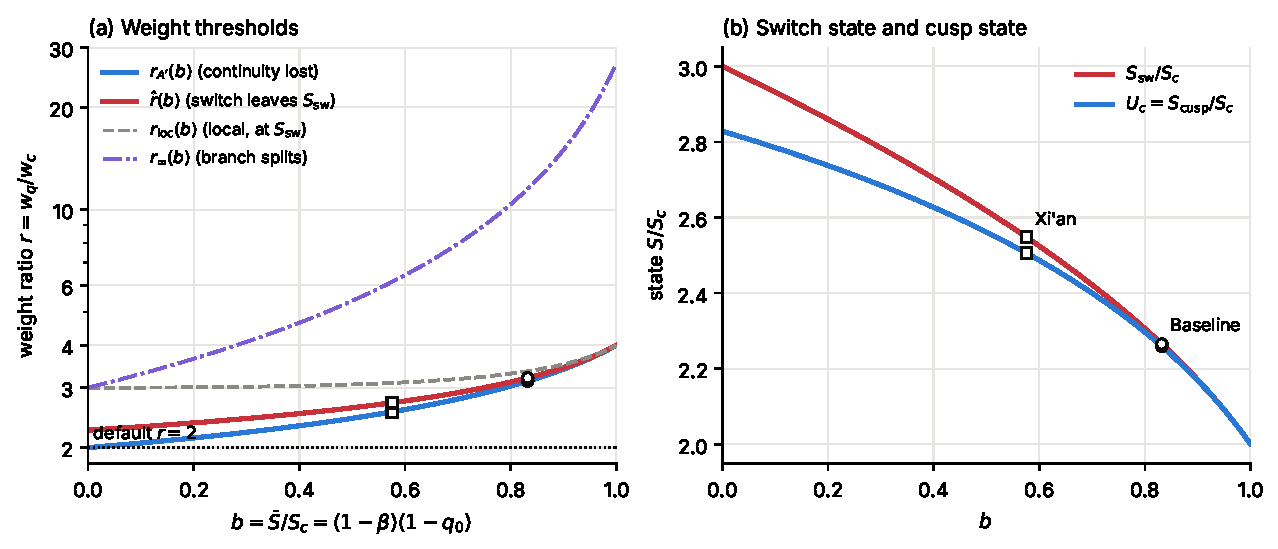
\includegraphics[width=\textwidth]{figs/F1_thresholds.pdf}
\caption{只依赖 $b$ 的阈值。(a) $\rA<\rhat<\rloc<\rinf$；点线为默认 $r=2$，圆点与方点为基准与西安参数。(b) $\Ssw/S_c$ 与尖点状态 $U_c$。}
\label{fig:thresholds}
\end{figure}

\begin{figure}[htbp]\centering
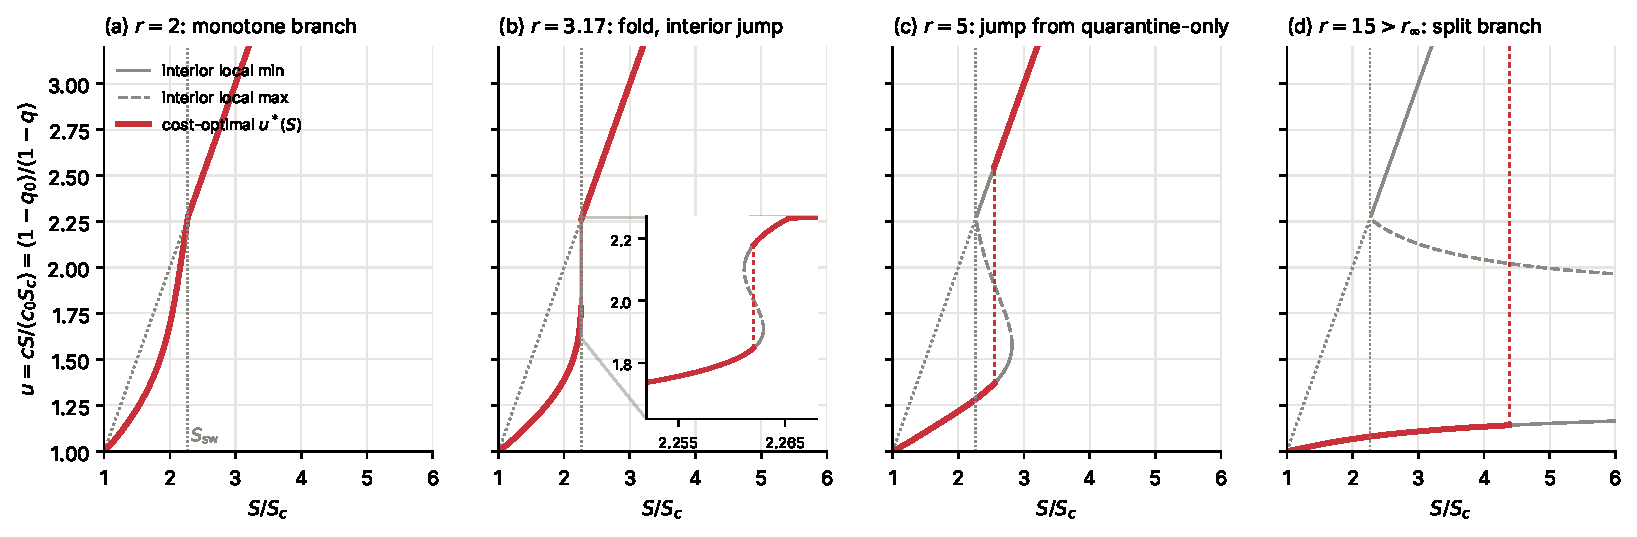
\includegraphics[width=\textwidth]{figs/F2_branches.pdf}
\caption{基准参数下的内部驻点曲线 $U=U_s(u)$（灰实线为局部最小、灰虚线为局部最大）、仅隔离控制 $u=U$（灰对角线；$U\ge\Ssw/S_c$ 时为局部最小）与成本最优路径（红线，虚线段为跳跃）。(a) $r=2$：曲线单调，控制连续。(b) $r=3.17\in(\rA,\rhat)$：曲线在 $u=2$ 附近折叠，产生一次内部跳跃（插图放大）。(c) $r=5>\rhat$：在 $S_{\rm glob}$ 处由仅隔离控制跳到下支。(d) $r=15>\rinf$：曲线断开。}
\label{fig:branches}
\end{figure}

\begin{figure}[htbp]\centering
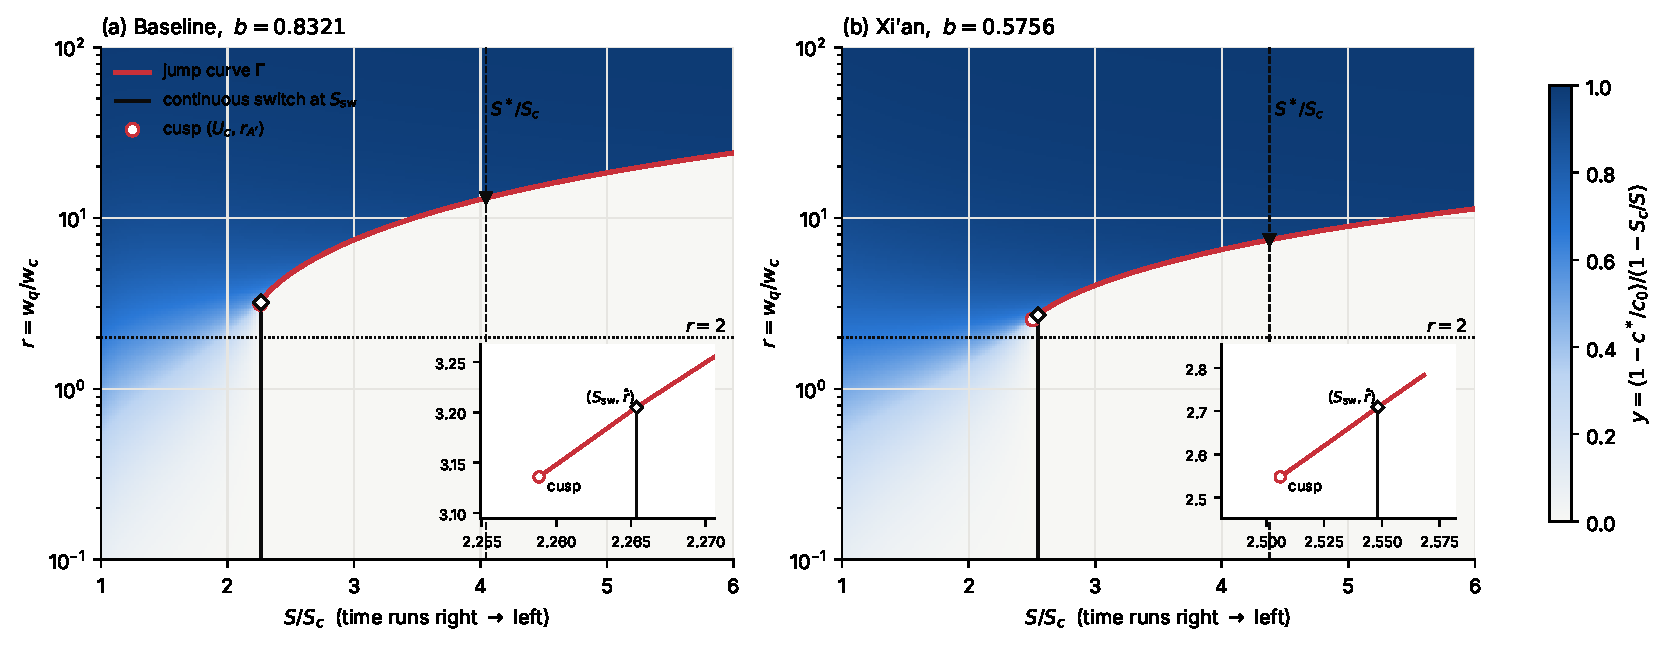
\includegraphics[width=\textwidth]{figs/F3_phase.pdf}
\caption{$(S/S_c,r)$ 平面上的成本最优控制。颜色 $y=(1-c^*/c_0)/(1-S_c/S)$：$y=0$ 为仅隔离控制，$y=1$ 为仅减少接触。红线为跳跃曲线 $\Gamma$；黑色竖线为 $r\le\rhat$ 时 $\Ssw$ 处的连续切换；白圆为尖点，菱形为 $(\Ssw,\rhat)$（插图放大）；竖虚线为 $S^*/S_c$，三角为 $r_C$。时间从右向左推进。}
\label{fig:phase}
\end{figure}

\begin{figure}[htbp]\centering
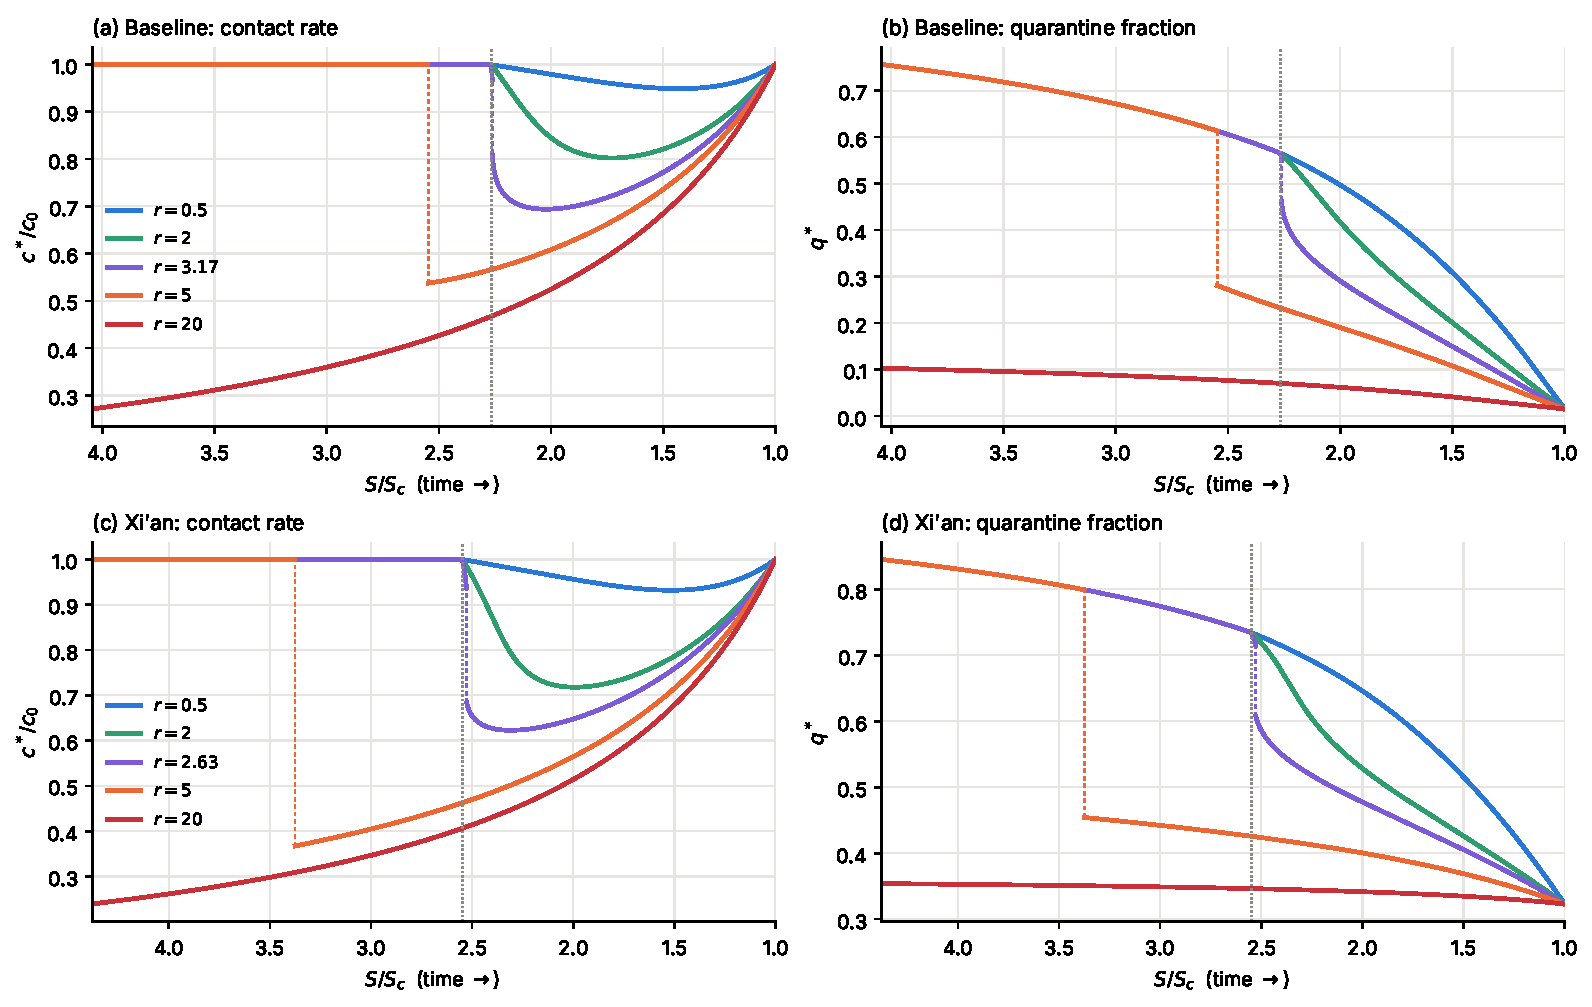
\includegraphics[width=\textwidth]{figs/F4_profiles_state.pdf}
\caption{代表权重下的成本最优控制（状态坐标）。基准：$r=0.5,2,3.17,5,20$；西安：$r=0.5,2,2.63,5,20$。竖直虚线为跳跃。$r=20>r_C$ 时没有仅隔离段。}
\label{fig:state}
\end{figure}

\begin{figure}[htbp]\centering
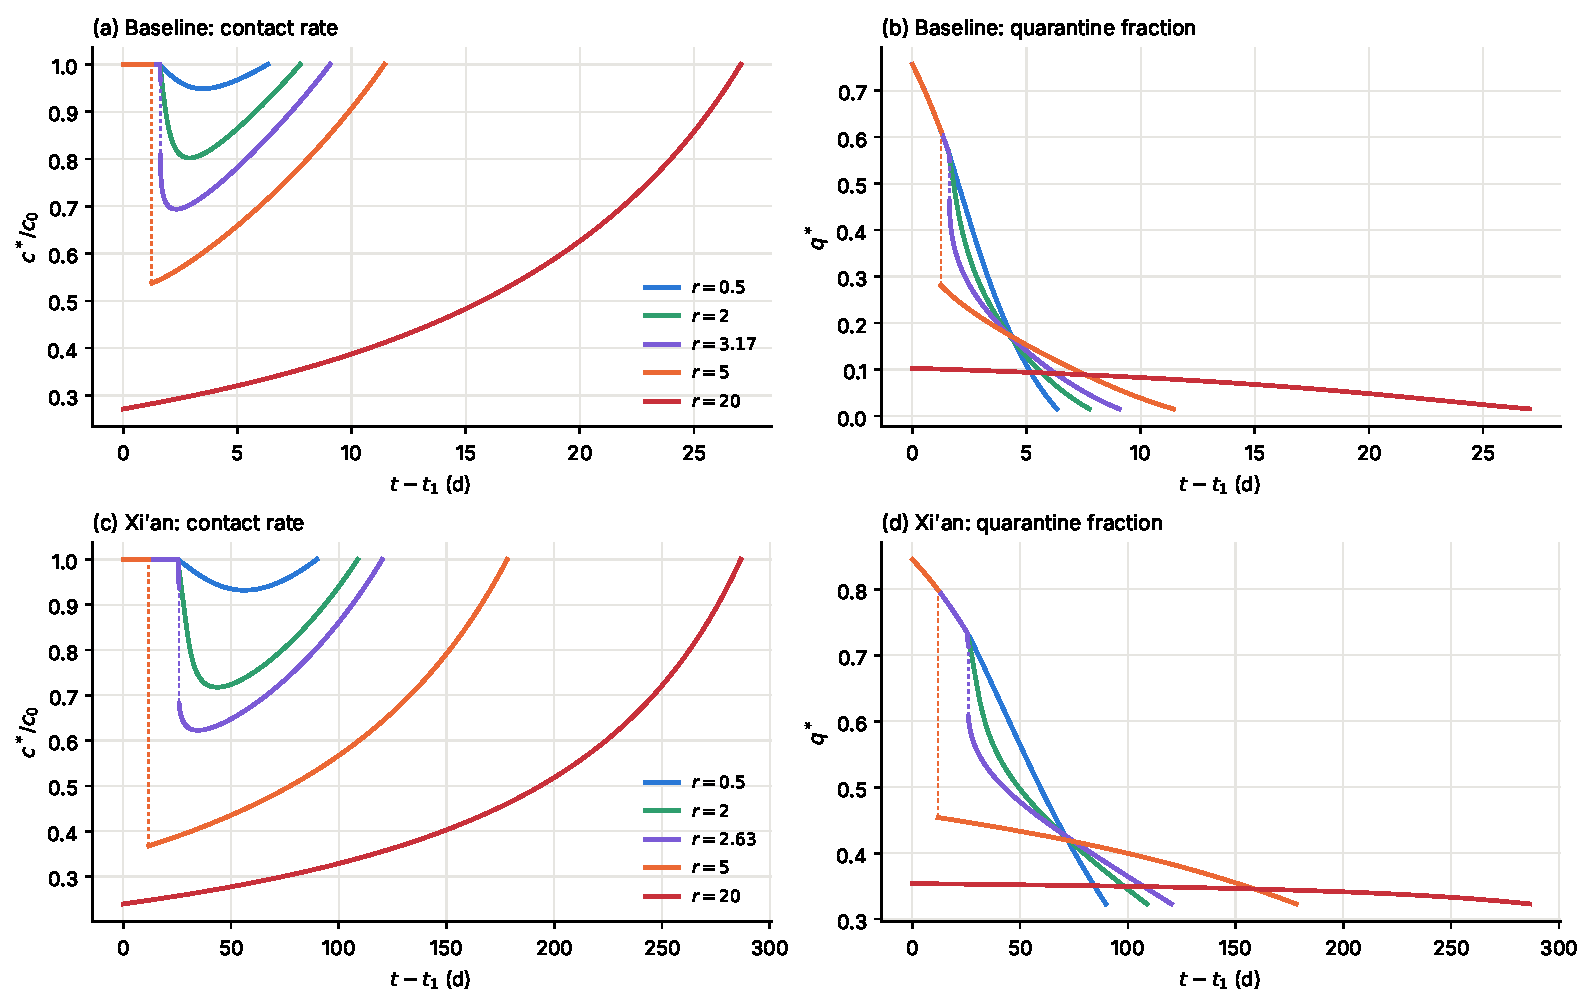
\includegraphics[width=\textwidth]{figs/F5_profiles_time.pdf}
\caption{与图~\ref{fig:state} 相同的控制，以 $t-t_1$ 为横轴。跳跃处隔离比例与接触率同时下降（定理~\ref{thm:monotone}(i)）。}
\label{fig:time}
\end{figure}

%==========================================================
\section{指标随权重的变化}
\label{sec:metrics}

由定理~\ref{thm:monotone}(ii)，加重隔离权重只会把控制推向减少接触：控制更长、感染更多、新增隔离易感者更少、成本更高但增长放缓（图~\ref{fig:metrics}，表~\ref{tab:metrics}）。尽管控制在 $\rA$ 以上有跳跃，各指标对 $r$ 仍连续：跳跃位置随 $r$ 连续移动，且在尖点处幅度为零。$r_C$ 处指标曲线出现折角，因为仅隔离段在这里消失。

\begin{proposition}[混合措施的代价与阈值无关]\label{prop:mixcost}\proven
记 $U_{\QO}(r)$ 为仅隔离段的起点（$r\le\rhat$ 时为 $\Usw$，否则为 $\Uglob(r)$）。若 $U^*\ge U_{\QO}(r)$，则成本最优控制与仅隔离控制之差为
\[
J_{\QO}-J_{\min}=\frac{w_cK(b,r)}{c_0\theta},\qquad
\Delta t-\Delta t_{\QO}=\frac{L(b,r)}{c_0\theta},\qquad
\Delta I_{\rm cum}=-\Delta S_q=\beta\bar S\,L(b,r),
\]
其中 $K=\int_1^{U_{\QO}(r)}[h(U)-G(u^*;U)]\,dU$，$L=\int_1^{U_{\QO}(r)}\bigl[\tfrac1{u^*-b}-\tfrac1{U-b}\bigr]dU$。多出的感染人数与 $\eta$、$S_0$、$I_0$ 都无关。由于 $h(U)\sim r/U$，仅隔离控制的成本随 $\ln U^*$ 增长，所以相对节省 $K/\!\int_1^{U^*}h\to0$（$U^*\to\infty$）。
\end{proposition}
\begin{proof}
在 $U\ge U_{\QO}(r)$ 上两种控制相同（定理~\ref{thm:upper}），差值只来自 $[1,U_{\QO}(r)]$，而那里的被积函数只依赖 $(b,r)$（引理~\ref{lem:invariance}）。感染与新增隔离易感者的差值由主稿定理 4.5 的仿射关系得到，系数为 $(1-\beta)\gamma\eta/(c_0\theta)=\beta\bar S$。
\end{proof}

$r=2$ 时，基准参数 $K=0.052671$、$L=0.925521$，西安参数 $K=0.070823$、$L=0.611789$。由此 $J$ 分别降低 $0.1053$ 与 $2.748$，$\Delta t$ 分别增加 $1.851$ d 与 $23.74$ d，感染分别多 $20.91$ 人与 $1.569\times10^5$ 人，都与主稿表 2 的差值一致。

\begin{figure}[htbp]\centering
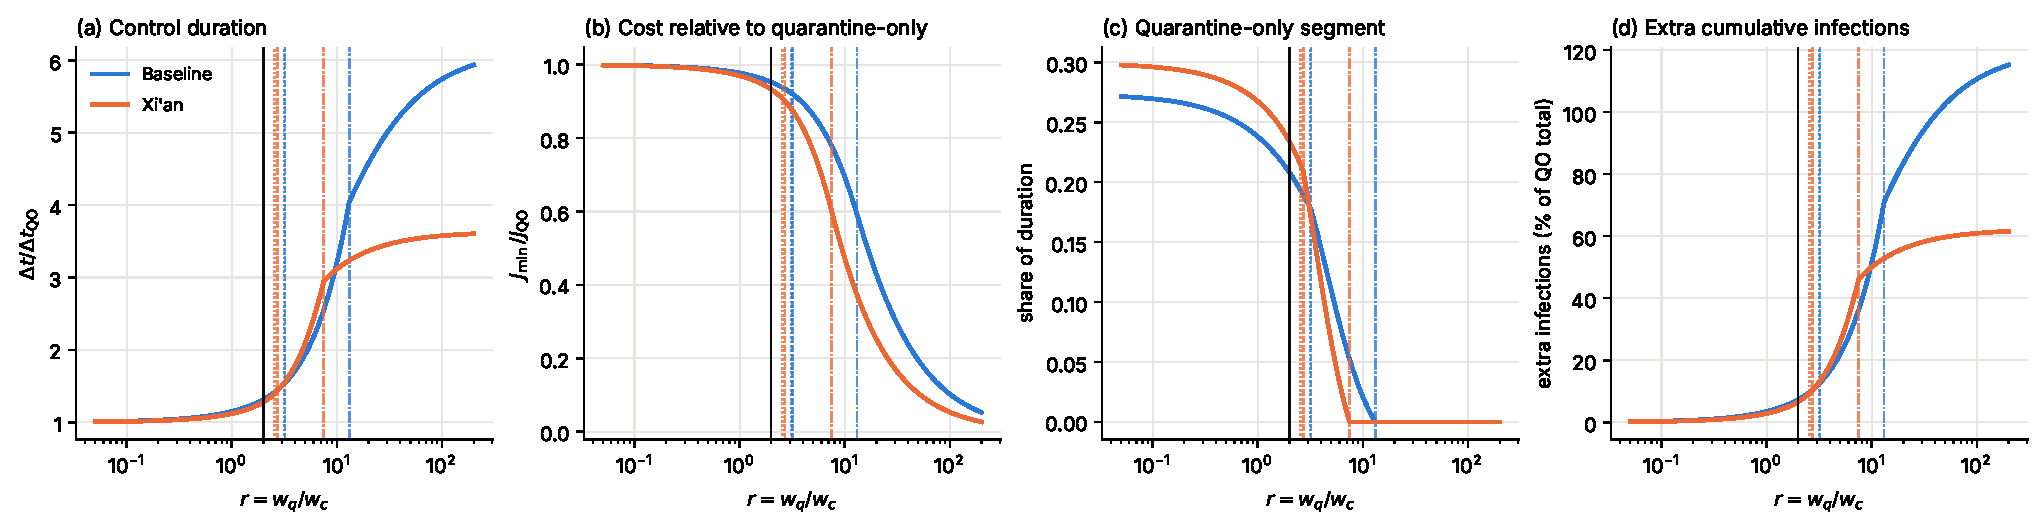
\includegraphics[width=\textwidth]{figs/F6_metrics.pdf}
\caption{指标随 $r$ 的变化（蓝：基准；橙：西安）。(a) 控制时长与仅隔离控制之比；(b) 最小成本与仅隔离控制成本之比；(c) 仅隔离段占控制时长的比例；(d) 总累计新增感染比仅隔离控制多出的部分，以后者的百分比计。竖线依次为 $\rA$（点线）、$\rhat$（虚线）、$r_C$（点划线），黑实线为 $r=2$。}
\label{fig:metrics}
\end{figure}

\begin{table}[htbp]\centering\small
\caption{代表权重下的指标（不考虑能力约束）。总累计新增感染计至清零；$S_q$ 为阈值控制期新增隔离易感者。$S_J/S_c$ 为跳跃状态，箭头为跳跃前后（$S$ 增大方向）的 $c/c_0$。}\label{tab:metrics}
\setlength{\tabcolsep}{4pt}
\begin{tabular}{@{}lrrrrrrl@{}}\toprule
$r$ & $\Delta t$（d） & $J_{\min}$ & $J_{\min}/J_{\QO}$ & 总累计感染 & $S_q$ & 仅隔离段（d） & 跳跃 $S_J/S_c$：$c/c_0$\\\midrule
\multicolumn{8}{@{}l}{基准参数（$N=763$，$\eta=0.05N$；人数单位为人；仅隔离控制 $\Delta t=5.903$ d，$J=2.2236$）}\\
0.5 & 6.331 & 0.5497 & 0.989 & 290.5 & 379.0 & 1.614 & —\\
1 & 6.780 & 1.0866 & 0.977 & 295.6 & 374.0 & 1.614 & —\\
2 & 7.754 & 2.1183 & 0.953 & 306.6 & 363.0 & 1.614 & —\\
$\rA=3.1358$ & 9.020 & 3.2127 & 0.921 & 320.9 & 348.7 & 1.614 & （尖点 2.2588，幅度 0）\\
$\rhat=3.2051$ & 9.104 & 3.2764 & 0.919 & 321.9 & 347.7 & 1.614 & 2.2654：0.790$\to$1\\
5 & 11.447 & 4.7983 & 0.863 & 348.3 & 321.2 & 1.254 & 2.5483：0.537$\to$1\\
10 & 18.901 & 7.7172 & 0.694 & 432.5 & 237.0 & 0.391 & 3.4741：0.345$\to$1\\
$r_C=13.102$ & 23.883 & 8.6163 & 0.592 & 488.8 & 180.8 & 0 & 4.0440：0.286$\to$1\\
50 & 31.847 & 10.834 & 0.195 & 578.8 & 90.8 & 0 & （10.49，在 $S^*$ 之外）\\\midrule
\multicolumn{8}{@{}l}{西安参数（$\eta=0.002N$；人数单位为 $10^6$ 人；仅隔离控制 $\Delta t=85.07$ d，$J=40.7686$）}\\
0.5 & 89.80 & 10.046 & 0.986 & 2.4092 & 7.9478 & 25.46 & —\\
1 & 95.20 & 19.769 & 0.970 & 2.4449 & 7.9121 & 25.46 & —\\
2 & 108.81 & 38.021 & 0.933 & 2.5348 & 7.8222 & 25.46 & —\\
$\rA=2.5477$ & 118.56 & 47.158 & 0.908 & 2.5993 & 7.7578 & 25.46 & （尖点 2.5060，幅度 0）\\
$\rhat=2.7090$ & 121.82 & 49.705 & 0.900 & 2.6208 & 7.7362 & 25.46 & 2.5483：0.646$\to$1\\
5 & 178.17 & 78.001 & 0.765 & 2.9932 & 7.3638 & 11.87 & 3.3759：0.367$\to$1\\
$r_C=7.4536$ & 250.72 & 91.791 & 0.604 & 3.4728 & 6.8843 & 0 & 4.3779：0.264$\to$1\\
10 & 265.15 & 96.154 & 0.472 & 3.5681 & 6.7889 & 0 & （5.44，在 $S^*$ 之外）\\
50 & 299.78 & 106.65 & 0.105 & 3.7970 & 6.5600 & 0 & （22.39，在 $S^*$ 之外）\\\bottomrule
\end{tabular}
\end{table}

%==========================================================
\section{能力约束}
\label{sec:capacity}

在 $u$ 坐标下，能力约束 $c\ge c_{\min}$、$q\le q_{\rm cap}$ 把允许区间收窄为
\[
\ell(U)=\max\{1,\ c_{\min}U/c_0\}\ \le\ u\ \le\ m(U)=\min\{U,\ (1-q_0)/(1-q_{\rm cap})\}.
\]

\begin{corollary}[截断规则]\label{cor:clip}\proven
若 $r\le\rA(b)$ 且可行性条件成立，则能力约束下的成本最优控制为 $u^*_{\rm cap}(U)=\min\{\max\{u^*(U),\ell(U)\},m(U)\}$，即把不考虑能力约束的成本最优控制截断到允许区间 $[c^-(S),c^+(S)]$。
\end{corollary}
\begin{proof}
单峰函数在子区间上的最小点就是无约束最小点在该区间上的投影（定理~\ref{thm:continuity}(i)）。$u$ 关于 $c$ 单调，所以在 $u$ 上截断等价于在 $c$ 上截断。
\end{proof}

$r>\rA$ 时 $G$ 不再单峰，截断不一定最优，但主稿定理 5.1 的有限比较仍然适用：候选为允许区间的两端点与区间内的五次方程实根。表~\ref{tab:cap} 用主稿图 6（6.4 节）的代表能力组合作核对。截断在 $r\le3$ 时与精确解一致；在 $r=5,10,20$ 时不一致，代价至多高出 $0.4\%$。原因是在 B 区段，不考虑能力约束时的前段是仅隔离控制；把它截断到 $q_{\rm cap}$ 之后，下支上的内部点可能更便宜。

\begin{table}[htbp]\centering\small
\caption{能力约束下的成本最优控制：截断规则与精确有限比较（基准 $c_{\min}/c_0=0.5$、$q_{\rm cap}=0.6$；西安 $c_{\min}/c_0=0.5$、$q_{\rm cap}=0.75$）}\label{tab:cap}
\begin{tabular}{@{}lccc@{\qquad}ccc@{}}\toprule
 & \multicolumn{3}{c}{基准} & \multicolumn{3}{c}{西安}\\
$r$ & $J$（精确） & $J$（截断） & $\Delta t$（d） & $J$（精确） & $J$（截断） & $\Delta t$（d）\\\midrule
0.5 & 0.70393 & 同左 & 6.916 & 12.3256 & 同左 & 97.74\\
1 & 1.27035 & 同左 & 7.364 & 22.4872 & 同左 & 103.15\\
2 & 2.36113 & 同左 & 8.338 & 41.6166 & 同左 & 116.75\\
3 & 3.38856 & 同左 & 9.443 & 58.5958 & 同左 & 135.94\\
5 & 5.21777 & 5.21791 & 12.079 & 85.5847 & 85.6303 & 166.96\\
10 & 8.72563 & 8.73497 & 16.073 & 143.0164 & 143.5825 & 184.02\\
20 & 14.89251 & 14.92606 & 17.865 & 252.7135 & 252.7308 & 191.04\\\bottomrule
\end{tabular}
\par\smallskip\footnotesize $r=2$ 时 $J$、$\Delta t$ 与主稿 6.4 节的 $2.361$、$8.34$ d 和 $41.62$、$116.8$ d 一致。
\end{table}

%==========================================================
\section{时长约束}
\label{sec:duration}

\begin{theorem}[凸前沿与乘子匹配]\label{thm:frontier}\proven
固定 $r$。全部允许控制的 $(\Delta t,J)$ 组成的集合是紧凸集，因而
\[
V(T)=\min\{J:\Delta t=T\}
\]
在 $[\Delta t_{\QO},\Delta t_{\rm contact}]$ 上是凸函数。对每个内点 $T$，存在 $\kappa\in-\partial V(T)$，以及使 $J+\kappa\Delta t$ 最小且 $\Delta t=T$ 的允许控制。若某些状态上的最小点不唯一，就在这些状态的一个可测子集上选用其中一个，以精确达到 $T$。$\kappa$ 是控制时长的影子价格；在不受时长约束的最优点上 $V'=0$，所以最小成本在其附近对时长不敏感。
\end{theorem}
\begin{proof}
在 $U$ 坐标下，$\Delta t$ 与 $J$ 都是控制值的有界函数对 Lebesgue 测度（无原子）的积分。由 Lyapunov 定理（Aumann 1965, J.\ Math.\ Anal.\ Appl.\ 12:1--12）：
\begin{itemize}
\item 可积有界、取闭值的集值映射的积分是紧凸集；
\item $\kappa$ 处全体最小点所能达到的 $\Delta t$ 值组成区间。
\end{itemize}
有界性来自 $u-b\ge1-b>0$。凸函数在内点有次梯度，取 $\kappa$ 为负的次梯度，由主稿注记 5.5 的不等式即得最优性。
\end{proof}

这补上了主稿注记 5.5 中“不保证每个允许时长都有匹配的 $\kappa$”的缺口。由于累计感染与新增隔离易感者都是 $\Delta t$ 的仿射函数，$V$ 同时就是 $J$ 与这两项指标之间的完整取舍曲线。图~\ref{fig:frontier} 是 $r=2$ 时的数值前沿：$\kappa$ 取 221 个值，每个状态网格 3001 点；所得前沿是凸的，且 $\kappa$ 随 $T$ 单调。

\begin{figure}[htbp]\centering
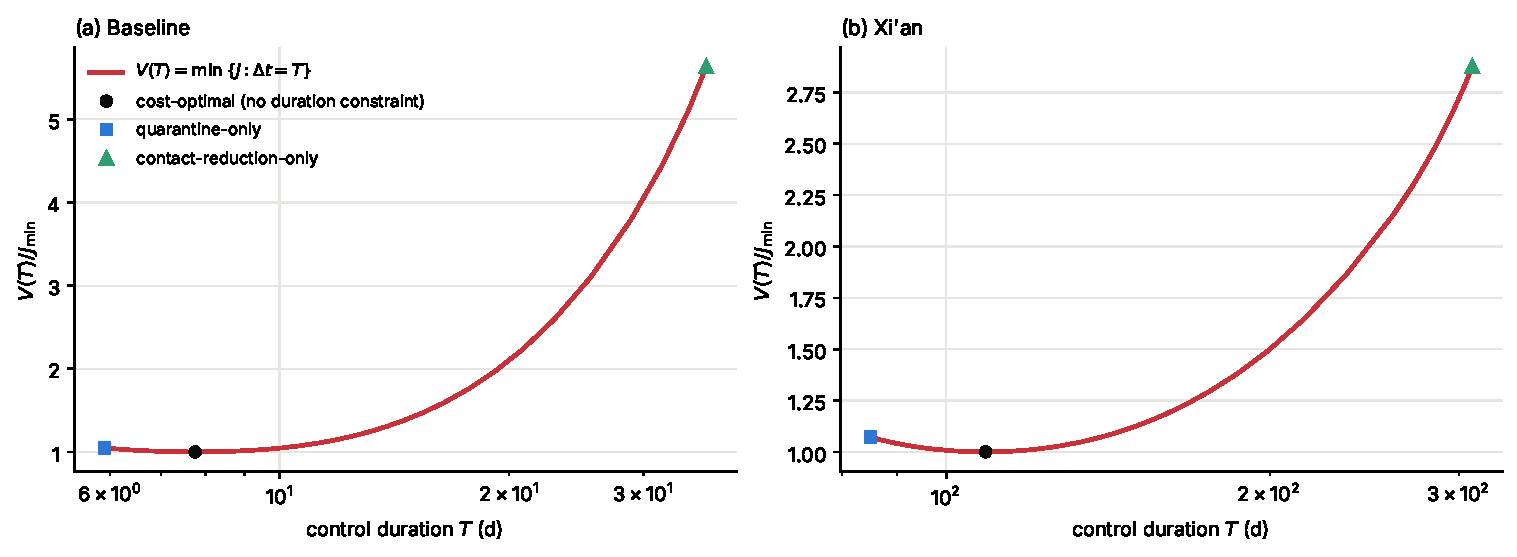
\includegraphics[width=0.95\textwidth]{figs/F7_frontier.pdf}
\caption{$r=2$ 时的最小成本 $V(T)$（以不受时长约束的最小成本 $J_{\min}$ 归一）。方点为仅隔离控制（基准 $1.050J_{\min}$，西安 $1.072J_{\min}$），三角为仅减少接触（$5.64J_{\min}$ 与 $2.88J_{\min}$）。}
\label{fig:frontier}
\end{figure}

%==========================================================
\section{小结：已经解决与尚未解决的问题}
\label{sec:open}

\textbf{已经解决的问题}（不考虑能力约束，无回流模型）：
\begin{itemize}
\item 所有权重阈值都只依赖 $b=(1-\beta)(1-q_0)$，并有闭式：$\Usw$、$U_c$、$\rA$、$\rhat$、$\rloc$、$\rinf$；$r_C$ 由一个三次方程给出。
\item 仅隔离段的起点 $S_{\rm glob}(r)$ 对一切 $r$ 都已刻画：$r\le\rhat$ 时为 $\Ssw$；$r>\rhat$ 时由有理参数化的相切条件确定，连续、严格增，并有下界 $\bar S+r(S_c-\bar S)$。
\item 连续性：控制在整个控制期连续，当且仅当 $r\le\rA$。此时最优控制唯一、单峰、有显式参数式，能力约束下只需截断。
\item 单调性：任意权重下隔离比例随时间不增；各指标随 $r$ 单调；$J_{\min}(r)$ 凹。
\item 时长约束：$V(T)$ 凸，每个时长都有匹配的乘子。
\end{itemize}

\textbf{只有数值证据的结论}：
\begin{itemize}
\item $r>\rA$ 时恰有一次跳跃，且跳跃点组成单调曲线 $\Gamma$（数值结果~\ref{num:onejump}、\ref{num:gamma}）；
\item $\Uglob(r)/[b+r(1-b)]\to1$；
\item 能力约束下截断规则在 $r>\rA$ 时的适用范围。
\end{itemize}
可能的证明途径是证明 $F_1(\cdot;b,s)$ 在 $(0,\sqrt{2\Usw-3})$ 上至多两次变号（对 $w$ 的六次多项式作 Sturm 计数，或用区间算术）。

\textbf{不在本文范围内的问题}：一般控制类中的最优控制；有限回流模型；能力约束下 $r>\rA$ 的完整结构（有限比较照样适用）。

%==========================================================
\appendix
\section{数值方法与核对}
\label{app:method}

\textbf{逐状态精确求解。} 对每个 $U$，候选为两个端点 $\{1,U\}$ 与五次多项式
\[
\bigl[-2(U-u)u^3+2rU^2(u-1)\bigr](u-b)-(U-u)^2u^3-rU^2u(u-1)^2
\]
在 $(1,U)$ 内的全部实根（与主稿定理 5.1 相同），取 $G$ 最小者。

\textbf{跳跃检测。} 先在 $U$ 网格上找出最小点的大幅变化，再二分 60–70 次；二分后两侧仍分离（差 $>10^{-6}$）的才记为跳跃，以排除尖点附近陡峭但连续的段。

\textbf{积分。} 按跳跃点与 $\Usw$ 分段，用自适应 Gauss–Kronrod 积分。

\textbf{独立性。} 全部计算独立于仓库代码：$S^*$ 由首次积分求根得到，不用 Lambert $W$。

\textbf{与已有结果的核对：}
\begin{itemize}
\item $r=2$：$\Delta t=7.7536$ / $108.807$ d，$J=2.11827$ / $38.0209$，$S_q=363.0$ / $7.8222\times10^6$，总累计感染 $306.6$ / $2.5348\times10^6$，与主稿表 2 一致。
\item 三个转折都落在 NR-3 的括区内（表~\ref{tab:thr}）：$\rhat$ 的闭式值与暴力二分相差 $<3\times10^{-8}$。
\item 能力约束代表点与主稿 6.4 节一致（表~\ref{tab:cap}）。
\item $P>0$ 的随机抽样：在 $1<u<\Usw$、$0<b<1$、$0<r\le2$ 上取 $2\times10^6$ 个点，$\min P/u^6=5.3\times10^{-6}$（最小值出现在 $b\to0$、$r\to2$、$u\to2$ 附近）。
\item $\operatorname{sign}U_s'=\operatorname{sign}F_1$：$4\times10^5$ 个随机点全部一致。
\end{itemize}

\textbf{脚本}（随稿附上，只依赖 numpy、scipy、sympy、matplotlib）：
\begin{itemize}
\item \texttt{core.py}：逐状态求解、阈值与跳跃定位；
\item \texttt{analysis.py}：阈值、跳跃曲线与指标；
\item \texttt{extra.py}、\texttt{extra2.py}：能力约束与时长前沿；
\item \texttt{figs.py}：作图；
\item \texttt{s2.py}–\texttt{s6.py}：符号核对（尖点、因式分解、$u=2$ 处的符号、伽罗瓦群、阈值次序）；
\item \texttt{t2.py}：$(b,r)$ 网格上的跳跃次数检验。
\end{itemize}

\end{document}
